

%%% BEGIN DISCUSSION %%%
\chapter{Discussion and Future Directions}

Collectively, our studies span diverse scales of investigation into ILC transcriptional regulation. Our microarray expression profiling study of the ILC1 and NK lineages focused on defining the regulatory responsibilities of a single transcriptional regulator, PLZF. Our single-cell expression profiling study of ILCP and \ab\UP{} ILC precursors expanded our purview and defined the developmental progression of many transcriptional regulators while refining our placement of ILC developmental branch points. Finally, our RNA-seq and chromatin accessibility profiling study of ILCP characterized the genome-wide influence ILC transcriptional regulators. 

%%% MICROARRAY CHAPTER DISCUSSION %%%
\section{Role of PLZF in ILC1 development}

The ILC1 and NK are phenotypically similar effector cells distinguished by expression of PLZF in ILC1 development. We compared the results from two contrasts, ILC1 to NK and ILC1 to PLZF-deficient ILC1, to determine the degree to which expression differences between ILC1 and NK cells can be explained by prior expression of PLZF in ILC1 development. In this way, we used a specific experimental design to establish that a majority of PLZF-dependent genes in ILC1 including Il7r$\alpha$ is part of the differentially regulated program between ILC1 and NK. 

Since this study represents a comparison between two contrasts, we point to the extension to multiple comparison analyses. For instance, in immune development many differentiating cell types can be influenced by single transcription factor or other perturbations. If we are interested in understanding the effect of perturbation in many contexts, we would be interested in the comparison of many related differential expression measurements. A method named CorMotif has been developed to jointly assess differential expression in many contexts simultaneously. CorMotif identifies and leverages patterns of shared differential expression between studies \cite{wei2014}, a strategy that has been demonstrated to increase statistical power in identifying eQTL in multiple tissues \cite{flutre2013}. We anticipate the use of these multiple comparison analyses will be increasingly useful as technical advancement in sequencing has reduced the cell requirements for transcriptional profiling and so greatly expanded the range of accessible cell types for comparison.

%%% SINGLE-CELL CHAPTER DISCUSSION %%%
\section{Single-cell transcriptional profiling of ILCP}

Through single-cell transcriptional profiling of ILC precursor populations we established a map of ILC developmental progression. This reconstruction was based on observable cell state heterogeneity among ILCP and \aLP precursor populations. By clustering single-cell transcriptional profiles of 100 immune factors, we could infer the sequence of developmental stages from continuity in expression of key regulatory factors and by profile similarity of adjacent clusters. We confirmed early induction of Id2, Nfil3 and Tox occurs among \aLP precursors and that the expression of PLZF and Tcf7 mark a transitional stage where LTiP branches from the ILCP. We also show that ILC lineage trifurcation occurs in the ILCP, and that ILC differentiation can occur through multi-lineage transcriptional priming. 

\subsection{Id2, Nfil3 and Tox mark the earliest stages of ILC development}

Early clusters comprised almost entirely of \aLP (cluster A) were marked by their expression of the early ILC developmental factors \textit{Id2}, \textit{Nfil3}, and \textit{Tox}. These clusters also did not express \textit{Zbtb16}, \textit{Tcf7}, or ILC effector markers corroborating their developmental placement prior to the ILCP. Ordering of these clusters further implied Id2 is the earliest expressed transcription factor, and is then followed by simultaneous induction of Nfil3 and Tox. These findings contrast suggestions that Nfil3 and Tox are responsible for the induction of Id2. This notion has been evidenced by the fact that Tox or Nfil3-deficiency leads to reduction in Id2 expression and that Id2 expression can rescue ILC-related defects in these backgrounds \cite{aliahmad2010,aliahmad2011,xu2015,male2014}. Further, Nfil3 has been shown to bind the Id2 promoter in CHILP and peripheral LTi. We note that these findings are not contradictory to Id2 expression that precedes Nfil3 and Tox. To account for all observations, early low-level expression of Id2 is likely later enforced and upregulated through positive feedback with Nfil3 and Tox. In our single-cell experiments we in fact observe increased transcriptional levels of Id2 following acquisition of Nfil3 and Tox. Further, if Nfil3 and Tox were to precede Id2 induction, we would have expected to observe a distinct group of cells that expressed Nfil3 and Tox but lacked Id2 expression. These observations might also be explained by possible discrepancies in Id2 transcript and protein expression levels, or by a difference in when Id2 is initially induced and when Id2 expression is required for developmental progression. While there is evidence that Nfil3 can regulate and potentially induce Tox, it is still unclear what factors or signaling are responsible for induction of Nfil3 and initial induction of Id2.


\subsection{Bifurcation of ILC and LTi cell branches}

We identified a transitional cluster (cluster B) composed of mixed aLP and ILCP that has particular relevance to branching between the LTi and ILCP lineages. While it was understood based on the developmental potentials of known precursors that LTi branching must occur prior to ILC differentiation, it was not clear where the common precursor to the ILC and LTi lineages would be found and what factors drive their bifurcation. The transitional cluster was marked by the earliest induction of \textit{Zbtb16} and \textit{Tcf7}, and was further characterized by expression of early ILC developmental factors including \textit{Id2}, \textit{Nfil3} and \textit{Tox}, while lacking expression of ILC differentiation markers. The partitioning of the cluster by \textit{Zbtb16} expression provided the indication that cells in this stage are poised to differentiate into LTiP, since \textit{Zbtb16} negative cluster B cells almost uniformly expressed \textit{Rorc} and were uniformly \textit{Gata3} negative. These \textit{Zbtb16} negative cluster B cells also did not express \textit{\Rora} and \textit{Cxcr5}, which are both expressed in more mature LTiP. The identity of this transitional cluster as the branch point of ILC and LTi is further corroborated by our single-cell culture experiments, which demonstrated that the late Flt3\UM{} \aLP stage is the last precursor that gives rise to both ILC and LTi. 

The expression profile of this transition cluster leads to the question of where EILP and CHILP precursors fit into this developmental progression. Since both \textit{Zbtb16} expressing and \textit{Zbtb16} negative cluster B cells express \textit{Tcf7} and cluster B represents the earliest induction of \textit{Tcf7}, the EILP would appear to be developmentally between the \aLP clusters and cluster B. The difficulty in placing the EILP derives from its lack of IL7r$\alpha$ expression, which is present on all known ILC precursors including the CLP. This suggests that an early ILC precursor with ILC, cNK and LTi potential transiently downregulates IL7r$\alpha$ to give rise to the EILP. Transient downregulation of IL7r$\alpha$ has precedence in both early T cell precursors as well as DP thymocytes in T cell development \cite{schlenner2010,allman2003,mazzucchelli2007}. Given that the original description of the CHILP is likely contaminated by ILCP and LTiP in the fetal liver, the question of where a true CHILP precursor to the ILC and LTi lineages would fit remains as well. We would expect this precursor to express high levels of Id2 and Tcf7 while not expressing PLZF and \RORgt. If these cells exist among Il7r$\alpha$\UP{} \aLP, it is surprising we did not observe them since we observe LTi primed late \aLP, although this could have been due to limited sampling in that developmental stage. Our clustering analysis and further investigations into dimensionality reduced representation of the single-cell transcriptional profiles suggest that late aLP cluster cells relatively contiguous with transitional cluster B cells. If the EILP and CHILP progress linearly between these stages, the fact that we do not observe a discontinuity between these clusters implies that we are not measuring enough alternate developmental factors that would corroborate the transition. An alternative possibility is that the downregulation of Il7r$\alpha$ and generation of the EILP and CHILP represent an alternative developmental pathway from the late aLP. The validity of these hypotheses need to be evaluated either through more extensive single-cell profiling that would incorporate an Il7r$\alpha$\UM{} EILP or through combined examination of Tcf7 and Id2 reporter strains. 

We can now construct a consolidated linear developmental scheme (Figure \ref{fig:dis_devscheme}) that merges transcriptional transitions determined through single-cell transcriptional profiling as well as those inferred from characteristics of other ILC precursors. In this model, we place the EILP immediately after the Flt3\UM{} \aLP following downregulation of Il7r$\alpha$ and upregulation of Tcf7. We then presume a bona fide CHILP precursor with high Id2 expression before upregulation of PLZF that gives rise to both LTiP and ILCP progenitors. From our single-cell transcriptional profiling, this specific placement of these precursor stages appears required for consistency with a linear developmental scheme. It will be important to corroborate this model.

%% Discussion Figure 1 Developmental Scheme %%
\begin{figure}[p]
\begin{center}
	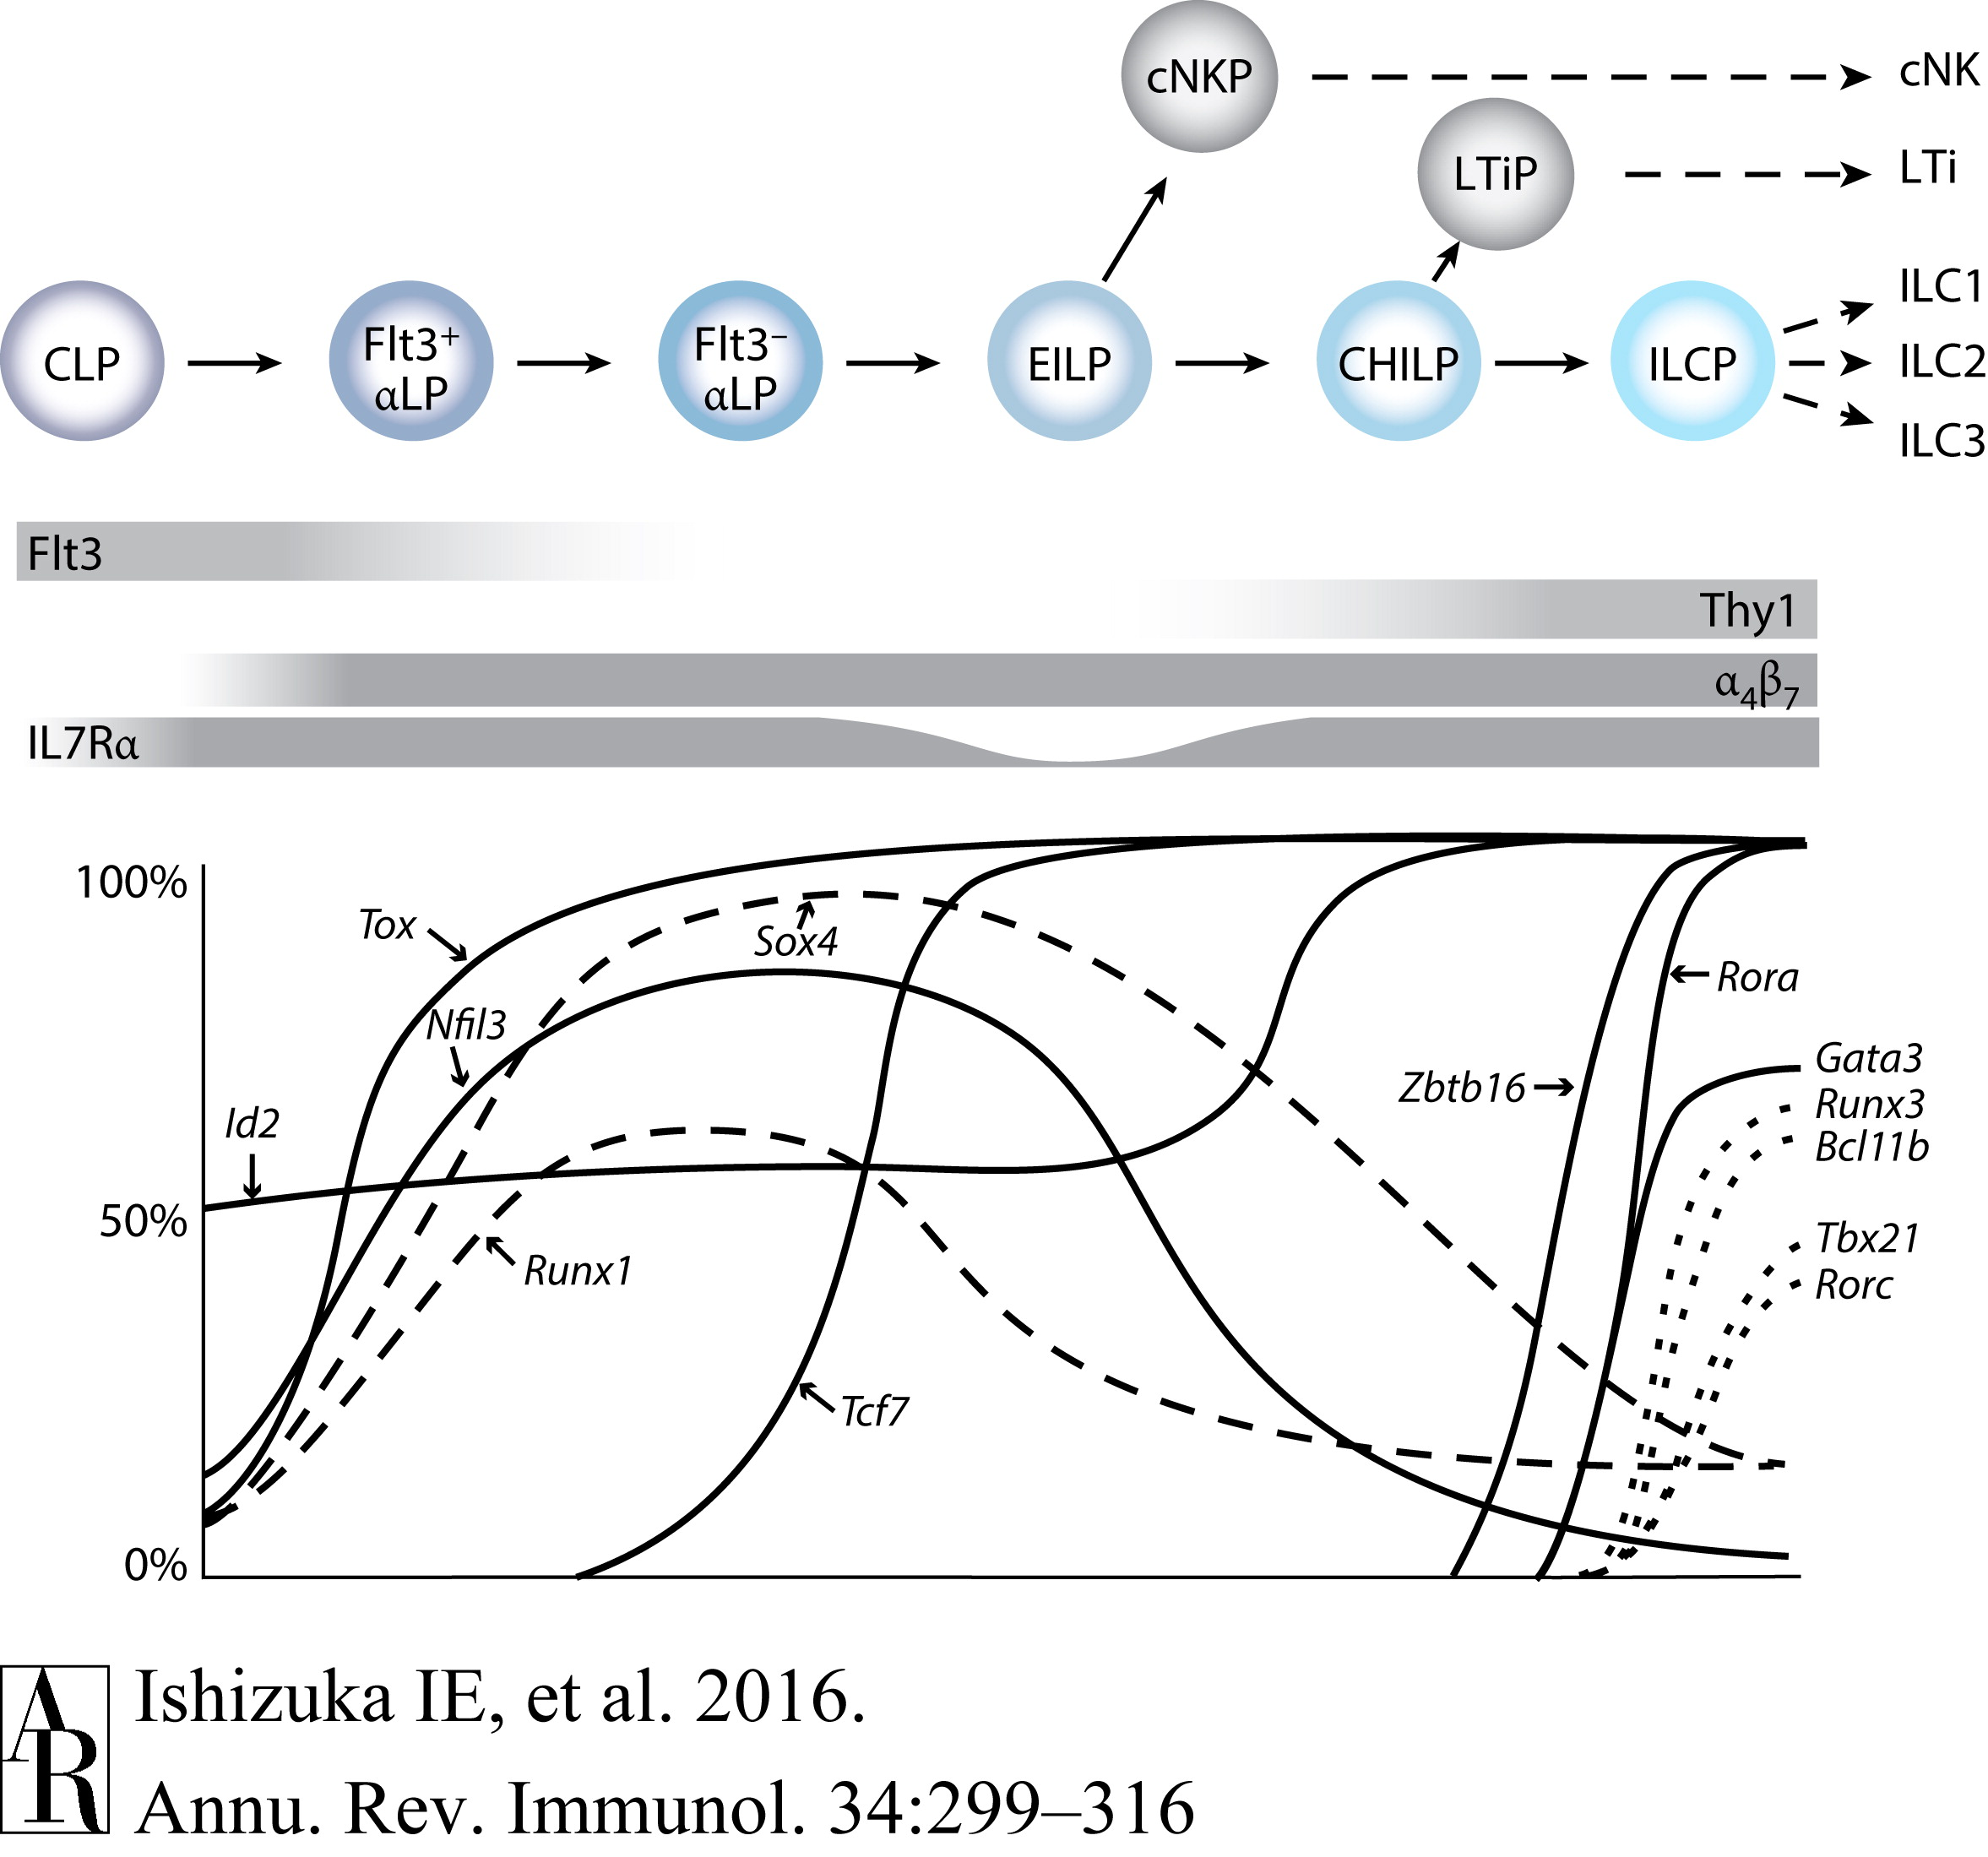
\includegraphics[width=0.7\textwidth]{figures/discussion/Discussion_1_development_scheme}
\end{center}
	\caption{Revised model of ILC developmental stages.} 
	(Top) Model depicting the stages of development from common lymphoid progenitor (CLP) to early (Flt3\UP) and late (Flt3\UM) \ab --expressing lymphoid precursor (\aLP), early innate lymphoid progenitor (EILP), common helper innate lymphoid progenitor (CHILP), and innate lymphoid cell precursor (ILCP). The conventional natural killer cell precursor (cNKP) and the lymphoid tissue inducer precursor (LTiP) are shown branching off of the EILP and CHILP, respectively. (Bottom) Sequential induction of transcription factors throughout ILCP ontogeny. The graph shows the percentage of cells positive for the indicated transcription factors as detected by single-cell transcriptomic analysis or transcription factor reporter strains \cite{ishizuka2016, yang2015}.
	\label{fig:dis_devscheme}
\end{figure}

\subsection{Lineage trifurcation and multilineage transcriptional priming}

Single-cell transcriptional profiling also established that initial ILC differentiation occurs in the ILCP. In fact, around half of ILCP express lineage-associated markers and many express markers associated with distinct lineages simultaneously. These multilineage transcriptionally primed precursors coexpressed \textit{Tbx21}, \textit{Gata3}, and \textit{Rorc}, in addition to other differentiation markers including \textit{Il2r$\beta$} (ILC1), \textit{Bcl11b} and \textit{Icos} (ILC2), and \textit{Lta}/\textit{Ltb} and \textit{Cxcr5} in mixed patterns. Similar coexpression of T-bet, Gata3, and \RORgt{} was observed in the Arg1\UP{} fetal intestinal ILC precursor \cite{bando2015}. Multilineage transcriptional priming during ILC development strongly contrasts direct polarization of T helper cell subsets by exogenous cytokine signaling during immune response \cite{zhu2010}. While these results demonstrate that ILC differentiation occurs through multilineage transcriptional priming, it does not appear to be a required developmental state. The fraction of multilineage primed precursors are dispersed throughout the dimensionality reduce ILC developmental trajectory. If all ILC precursors pass through a multilineage primed state, we would expect these cells to be tightly grouped and form a distinct state. This suggests that multilineage transcriptional priming in ILCP is stochastic process, either induced transcriptionally or through exogenous signals. Interestingly, the mixed patterns of multilineage priming imply that all combinations of lineages need to be resolved into individual fates. 

\subsection{Transcription factor expression profiles}

Single-cell transcriptional profiling revealed precise stage specific patterns of expression for known and novel transcriptional regulators. Gata3 is promiscuously expressed at the ILCP stage and can be found at intermediate to high levels in roughly 70\% of ILCP by staining \cite{constantinides2014}. By multiplex qPCR we observed \textit{Gata3} transcript expression in about half of ILCP, but in diverse transcriptionally primed states, further corroborating that Gata3 is not strictly associated with the ILC2 fate in development. Similarly, we observed \textit{\Rora} expression in almost all ILCs following induction of PLZF as well as in LTiP. While Gata3 deficiency results in defects in all ILCs as well as LTi, Rora deficiency only affects the generation of ILC2s \cite{halim2012}. We also observed close association of \textit{Bcl11b} and \textit{Rxrg} expression with the ILC2 primed ILCPs, indicating that the two transcription factors are early markers for ILC2 commitment. Conditional deletion of Bcl11b has confirmed that loss of Bcl11b blocks ILC2 development at the ILCP stage \cite{yu2016}. Any specific role of Rxrg in ILC development is unknown. \textit{Irf8} appeared to be preferentially associated with \textit{Tbx21} primed ILCPs, although any role it has is also unknown. The transcription factors \textit{Sox4} and \textit{Runx1} were both transiently expressed and induced just prior to expression of PLZF. The peak expression of these factors is suggestive of the possibility that they may influence the bifurcation of LTi and ILCP. Known targets of Runx1 including Id2, Ets1 and Sox4 are all upregulated at the transitional cluster B stage. In T cell development, Runx1 has been shown to enhance \RORgt{} expression and negatively regulate Gata3, implying a capability to influence LTi \cite{lazarevic2011}. Similarly, Sox4 is also capable of upregulating \RORgt{} and repressing Gata3 \cite{kuwahara2012}.

In aggregate, our current understanding of ILC lineage-specific regulators is sufficient to provide an initial picture of how lineage differentiation is likely enforced (Figure \ref{fig:dis_network}). The early requirement of Notch signaling for ILC2 development draws analogy to the Notch-Tcf7-Gata3-Bcl11b cascade established in thymocyte development \cite{Rothenberg2013}. Although Notch signaling does not appear to be required for Tcf7 upregulation in ILC precursors, it may still play a role in enforcing expression of Tcf7 expression as well as subsequent expression of Gata3 and Bcl11b. Downstream of Tcf7, it is apparent that transcription factors Gata3, Bcl11b and Gfi1 form a positive reinforcement loop for the ILC2 lineage. The ILC2 associated regulators Gata3 and Gfi1 have well-established roles in suppressing genes associated with Th1 and Th17 differentiation. Among transcription factors, Gfi1 directly inhibits Sox4 \cite{Zhu2006,Zhu2009} while Gata3 antagonizes Runx3 at the protein level and may indirectly inhibit expression of T-bet \cite{yagi2010}. In the inverse direction, Runx3 antagonizes Gata3 at the protein level and T-bet can suppress Gata3 expression. It is apparent that these lineage-enforcing mechanisms are only representative of cross-inhibition between ILC2 and ILC1/3 programs, and further investigation is required to establish whether ILC1 and ILC3 lineages also enforce their bifurcation.

%% Discussion Figure 2 Developmental Scheme %%
\begin{figure}[h]
\begin{center}
	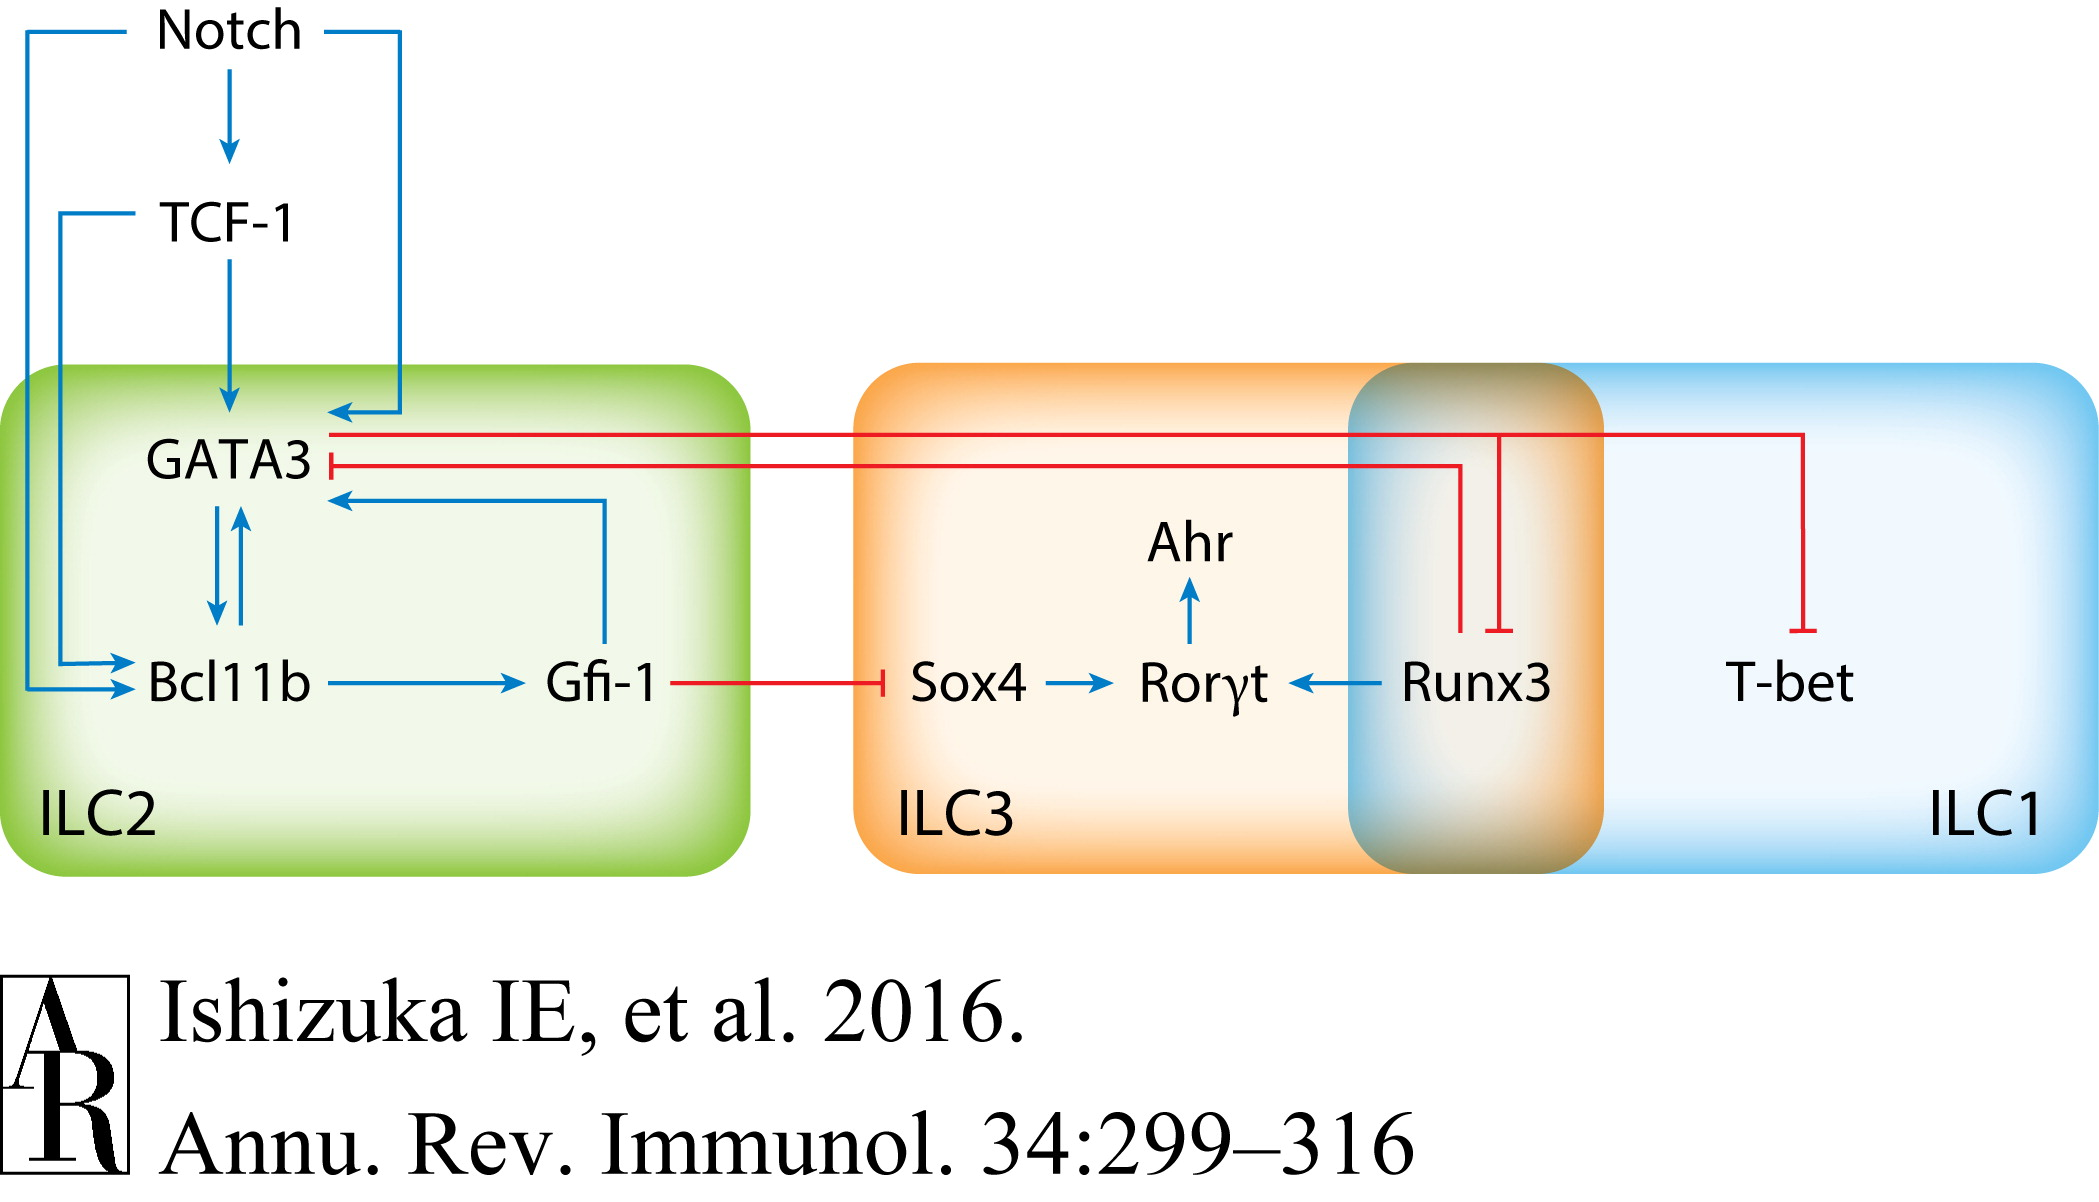
\includegraphics[width=0.5\textwidth]{figures/discussion/Discussion_2_network}
\end{center}
	\caption{ILC lineage transcription factor network.} 
	Transcription factor networks regulating cytokine effector programs in innate lymphoid cell (ILC) lineages. Blue arrows depict positive interactions, whereas red lines depict inhibitory interactions at the gene or protein level.
	\label{fig:dis_network}
\end{figure}

\subsection{Requirements for ILC differentiation and development}

It is informative to view the observed characteristics of ILC differentiation through the lens of ILC developmental requirements. As the roles of ILCs are further defined, it will become important to understand what specific properties of the collective innate immune system need to be maintained for effective immunity. Besides functionality in individual ILC lineages, it has been demonstrated that modulation of relative cell numbers of ILC2 and ILC3 lineages is important for type-specific pathogen clearance in the periphery. Accordingly, we might expect that it is important to achieve full representation of required peripheral ILC types in acceptable proportions. If particular ratios of ILC cell types require regulation, the natural extension is to consider whether this imposes constraints on ILC development. It is apparent that dietary ligands such as AhR ligands and retinoic acid can modulate the sizes of peripheral pools of ILCs in the intestine, although it is unclear if these peripheral expansions require contributions from hematopoietic-compartment ILC progenitors. Parabiotic mice studies have demonstrated that there is minimal replacement of tissue-resident ILCs by circulating hematopoietic cells over the timescale of weeks, although inflammatory conditions promotes some recruitment of presumably newly generated bone-marrow derived ILC2 cells \cite{Gasteiger2015}. This suggests that the peripheral balance of ILC types can be primarily maintained through expansion and contraction of differentiated ILC populations, which would imply that developmental output from hematopoietic ILC progenitors does not need to be strictly regulated. Instead, if hematopoietic ILC progenitors are mostly required for re-population of specific lineages during inflammatory stress, modulation of ILC developmental output by external signals might be a stronger developmental requirement than proportional generation of ILC types. A more general demonstration of compensation among components of the innate immune system can be seen in a study of patients with severe combined immunodeficiency. Although stem cell transplants reconstituted B, T, cNK and ILC1 cells but not ILC2 and ILC3 cells, these patients did not contract common herpes virus at higher rates \cite{vely2016}.

Given the slow turnover of peripheral tissue-resident ILCs, perhaps the most crucial phase of ILC development is the seeding of peripheral tissues from fetal ILC progenitors. The importance of the initial embryonic waves of ILCs and related lineages is best exemplified by the strict requirement for the LTi lineage in embryonic development. Inadequate generation of LTi precursors associated with maternal retinoid deficiency ultimately results in insufficient production of secondary lymphoid structures and permanently impaired immune fitness \cite{van2014}. Interestingly, this retinoic acid dependent generation of fetal LTi precursors is accomplished through expression of \RORgt, which is almost entirely absent in adult ILC precursors. The existence of distinct developmental hierarchies in fetal and adult hematopoiesis has precedence in upstream differentiation of the HSC, where potential for erythroid and megakaryocytic lineage branching occurs throughout the early cellular hierarchy in the fetus but is restricted to the stem cell compartment in the adult \cite{notta2016}. In the fetus then, it is important to ensure that regulation of the developmental choice between the LTi and ILC lineages results in sufficient numbers of LTi. Further investigation is required to determine whether this developmental decision is actively monitored through feedback via retinoic acid or other molecules, or if adequate LTi cell numbers are achieved passively in development. Among other ILC lineages however, there are not strong reasons to believe that their differentiation is strictly regulated aside from the requirement that all ILC types are generated in the fetus for seeding peripheral cells. 

This interpretation of ILC developmental requirements can shape our understanding of ILC developmental stages. Generally speaking, in transit from a multipotent stem cell to a differentiated effector cell, we should expect that intermediate developmental stages are only strictly required if sequential induction of lineage-specific factors is necessary or if input signaling is needed to make an appropriate developmental branching decision. In ILC development, transit through the early sequence of Id2, Nfil3, and Tox induction prior to ILC differentiation might be necessary for proper divergence from the adaptive lymphoid lineages and upregulation of Tcf7 and PLZF. Given that development of LTi is responsive to retinoic acid signaling and required in embryonic development but dispensable in adult, we would anticipate there is a necessary developmental stage that processes the decision between LTi and ILC lineages. However, if the downstream differentiation of ILC1, ILC2 and ILC3 lineages does not require strict regulation as suggested above, then the differentiation process could be resolved through a variety of developmental paths rather than through a rigid developmental sequence. 

In fact, a few characteristics of multilineage transcriptional priming observed in ILCP support the notion that ILC differentiation may be resolved non-deterministically. First, we observed all combinations of ILC lineage master regulators (\textit{Tbx21}, \textit{Gata3}, and \textit{Rorc}) among multilineage transcriptionally primed cells in ILCP. This includes tri-lineage primed cells as well as all possible combinations of bi-lineage primed cells, which implies that all possible ILC lineage bifurcations are resolved during differentiation. Second, dimensionality reduction based visualization of the ILC developmental path revealed that all types of multilineage primed precursors are interspersed throughout ILC differentiation rather than tightly grouped, as might be expected if a multilineage primed state was a required developmental stage. Moreover, multilineage priming appeared to be possible even in cells ostensibly committed to a particular lineage, as a few ILC2 primed cells that express \textit{Gata3}, \textit{Bcl11b}, \textit{Icos}, \textit{Il13}, and \textit{Il1rl1} could still be found with \textit{Tbx21} or \textit{Rorc} expression. This observation is more consistent with sporadic generation of multiple lineage regulators rather than a developmental model where multilineage regulator competition must be first resolved before further differentiation. 

Stochastic fluctuations of lineage regulators has precedence in both early HSC differentiation and in embryonic stem cells \cite{pina2012,abranches2014}, and multiple developmental paths to particular lineages has also been observed in early HSC differentiation \cite{pina2012,notta2016,laslo2006}. We will note that the suggestion that the resolution of three ILC lineages occurs through stochastic competition between lineage regulators is uniquely representative of a lineage trifurcation, where restriction of developmental potential is typically thought of as successive bifurcations. Among ILC lineages, the spectrum of functional plasticity between the ILC1 and ILC3 lineages as well as the observed cross-inhibition between ILC2 and ILC1/3 factors might be indicative that resolution of the bifurcation between the ILC2 and ILC1/3 lineages is most important.

The widespread expression of lineage-defining transcription factors Gata3 and \RORgt{} in early ILCP further speaks to the unconstrained nature of ILC differentiation. Both of these transcriptional regulators are expressed immediately following acquisition of PLZF and are observed simultaneously with the expression of genes associated with all lineages. Despite posited roles of these factors in inhibiting competing lineages, it seems likely that these cross-inhibitory mechanisms might be effective only in later stages of differentiation given the degree of multilineage transcriptional priming observed. Modulation of the strength of these inhibitory interactions could be realized through a few mechanisms. Cross-inhibition could depend on the activity of other mediating proteins, for example indirect inhibition of \RORgt{} by Gata3 could be primarily mediated through inhibition of Runx3. Modulation of the epigenetic enhancer landscape could also adjust the degree to which transcription factors influence their downstream targets. As an example, the regulatory enhancer landscape surrounding ILC2 effector genes Il4, Il5 and Il13 shifts through progression from ILCP through ILC2P to peripheral ILC2s, presumably corresponding to regulatory enforcement of the lineage. Further investigation is needed to see if similar regulatory adjustments occur around developmental transcription factors as well.

The developmental requirements for ILC differentiation also appear less stringent in comparison to other studied developmental systems. Among the hematopoietic compartment, the development of the adaptive B and T cell lineages requires specific coordination with recombined receptor signaling. Since the specificity of recombined antigen receptors cannot be anticipated, developing B and T cells must repeatedly assess receptor gene rearrangement status and signaling competence at distinct developmental checkpoints \cite{rothenberg2014}. Furthermore, the measured signaling specificity at these required developmental checkpoints determines whether development can proceed and which cell fates are accessible. Both adaptive B and T cell lineages sequentially rearrange the two component chains of their antigen receptors in a strictly specified developmental progression to test for successful gene rearrangement, guard against self-reactivity, and, for T cells, ensure sufficient specificity for antigen-presenting molecules \cite{melchers2015,carpenter2010}. As another illustration, \abT cells differentiate into helper (CD4\UP) and cytotoxic (CD8\UP) T cell subsets whose functions depend on recognition of two different classes of antigen presenting molecules MHCII and MHCI, respectively. Accordingly, the CD4-CD8 lineage decision must match receptor specificity to MHCII or MHCI, and is accomplished through a specific progression from a CD4\UP CD8\UP{} double-positive cell state that essentially tests whether downregulation of coreceptor CD8 influences receptor signaling. Other antigen receptor specificities results in the production of other lineages, for example the expression of particular invariant chain antigen receptors with specificity to MHC class I-like Cd1d results in the differentiation of invariant NK-like T cells \cite{egawa2005} while self-reactivity in the thymus can lead to differentiation of CD4\UM CD8\UM{} double-negative TCR$\alpha\beta$ IELs and regulatory T cells \cite{mcdonald2014,stritesky2012}. In other well-studied non-hematopoietic developmental systems, such as zygote development and intestinal crypt formation in mammals as well as retinal neuron specification and embryonic stripe formation in Drosophila, cellular differentiation is strongly constrained by spatial relationships that must to be maintained among differentiated cells, granted these systems are typically studied for their precise developmental regulation. In these systems, imprecise lineage specification of adjacent cells can lead to functional defects, which is typically not of concern among mobile hematopoietic cells.

\subsection{Considerations in single-cell transcriptional profiling analysis}

Overall, our analysis of single-cell transcriptional profiling of ILC precursors is demonstrative of the many advantages single-cell studies possess compared to population-level transcriptional studies. From a heterogeneous ILC precursor population, we isolated a previously unaccounted for mast-like contaminating population. With the remaining single-cell profiles, we were able to construct a developmental progression of transcriptional states and identify the branch point of LTi and ILCp as well as the stage of ILC lineage trifurcation. Our developmental progression uncovered transient expression dynamics of important transcription factors including Nfil3, Runx1 and Sox4, all of which are missed in population-level transcriptional profiling of CLP and ILCP. Single-cell transcriptional profiles at the stage of lineage trifurcation revealed that individual ILC precursors undergo multilineage transcriptional priming, which could not be inferred from population-level profiling. Further representation of our developmental trajectory using a dimensionality reduction based approach revealed the limitations of a clustering based strategy. In our clustering analysis, individual ILC lineage branches were not resolved but rather clustered together according to their degree of maturity. In our dimensionality reduced representation, developmental maturation as well as individual ILC differentiation branches could be resolved simultaneously. The single contiguous picture of developmental stages that a single-cell study produces is very informative for the interpretation of precursor relationships, since it imposes restrictions on where precursor snapshots can potentially reside. 


Our observations in producing developmental pathway representations of single-cell transcriptional profiling data point towards several ways these analyses might be improved or extended. A relatively new technical challenge in the analysis of single-cell data is the prevalence of expression dropout events, or transcript levels below the limit of detection. In our single-cell multiplex qPCR data we can clearly observe measurement artifacts in the low expression regime, which indicate that complete dropout events are also likely. Appropriate accounting for dropout noise will likely need to be specific to the single-cell technology used as different measurement methodologies have different transcript sampling characteristics. In the case of technologies like single-cell multiplex qPCR and mass cytometry with a targeted set of genes assayed, we imagine noise models will need to be assay and probe specific. Expression dropout events can be accounted for with a zero-inflated expression model, where the distribution of expression values is assumed to be a explicit mixture of zero values for dropout events and of a second continuous distribution for measurable expression. For single-cell qPCR data, there has been some work that suggests treating expression dropout explicitly with a zero-inflated expression model increases statistical power in differential expression analysis \cite{mcdavid2012,kharchenko2014}. For single-cell RNA-seq data, a few studies have developed mathematical models to explicitly deconvolve the relative contributions of technical and biological variability in expression measurements \cite{brennecke2013,grun2014}. A recent intriguing suggestion for single-cell RNA-seq is to simultaneously perform clustering, normalization and dropout imputation, essentially contextualizing noise model to specific cell subpopulations \cite{azizi2017}. Importantly, explicit noise modeling in these datasets will be necessary to establish the degree to which measured heterogeneity reflects true biological variability. By extension, this detailed expression modeling might also need to be considered in interpretation, as they could indicate that particular developmental transitions are unresolvable if dominated by technical noise.

In the study of continuous developmental transitions, there have been recent shifts in how to represent and interpret these processes from single-cell expression data. Dimensionality reduction techniques for single-cell expression data typically produce a visualization of developmental paths in two dimensions by default. We note that in our ILC differentiation data, there is evidence of a potentially non-deterministic lineage trifurcation. The three differentiation possibilities with expression profile representation among all possible bilineage combinations would require at least three dimensions for representation of all developmental paths, although we expect the two dimensional projection highlights the predominant lineage relationships. Developmental paths are also typically represented linearly, where sampled cells are assigned a single pseudotime metric that infers their placement earlier or later in differentiation. The sporadic representation of multilineage ILC states would suggest that higher-dimensional structures might be more representative of developmental transitions rather than linear paths, particularly at differentiation decisions. In other words, particularly around loosely regulated differentiation decisions, it may be more accurate to consider the set of potential developmental trajectories that result in lineage specification rather than the average linear trajectory. In fact, within the remaining variability surrounding linear developmental paths, it would not be surprising to find possibly parallel developmental trajectories. More explicit physical modeling of the molecular components on developmental paths could best inform what trajectories are possible and has been demonstrated to some degree in dynamical systems based models of lineage bifurcations and transitions with single-cell data \cite{marco2014,morris2014}. These dynamical systems models can be further informed by incorporating restrictions on the true timescale of expression dynamics for different genes as well as by incorporating information that establishes the developmental potential observed in different regions of a trajectory. 

In current developmental trajectory analyses, lineage branches are assumed to diverge rather than reconnect at downstream points. However, the discussion above suggests that developmental trajectory analyses may need to accommodate divergent paths to common differentiated states, or developmental cycles. In our ILC data, we observe distinct lineage branching for the phenotypically similar LTi and ILC3 lineages. Furthermore, the anticipated expression profiles of EILP and CHILP entertain the possibility of alternative developmental paths prior to generation of the ILCP. Alternative developmental paths also have precedence in early HSC differentiation, as discussed above. It should not be difficult to extend branching analyses to handle lineage convergence, as branching detection methods could be simply applied along the reverse developmental trajectory of a differentiated lineage that converged.


In the future, single-cell trajectory analysis should focus on enhancing the analysis of genes that govern cell state transitions. The first step towards this goal is the identification of differentially expressed genes along continuous developmental trajectories. This differential expression problem is fundamentally different from the typical design in bulk microarray or RNA-seq experiments, where discrete pairs of conditions are typically compared. Differential expression along developmental trajectories requires statistics that reveal the association of a gene’s expression with a continuous developmental pseudotime-like metric. We also anticipate there will increasingly be experimental designs in which developmental trajectories are compared following perturbation of a gene or change in  condition. The comparison of continuous trajectories is very different from bulk differential expression since we are interested in understanding how lineage paths are shifted or truncated, as observed following perturbation of Bc11b in ILC precursors \cite{yu2016}. For these comparisons, we would imagine it might be necessary to pair equivalent regions on developmental paths to contextualize any differential expression that may be present. To determine how genes govern cell state transitions, we anticipate there will be substantial computational focus on regulatory network reconstruction based on the ample cell state transition data provided by single-cell trajectory reconstructions. The accessibility of bulk expression profiling data initially led to substantial interest in regulatory network reconstruction, although these efforts were ultimately stymied by insufficient samples for inference across thousands of genes as well as the substantial variability lost in bulk averaging. Accordingly, the large datasets being generated for high-dimensional expression states in single cells makes single-cell expression profiling studies an attractive prospect to revisit the network reconstruction problem. A few studies already demonstrate initial efforts into network reconstruction strategies, including a Boolean switch-based network model \cite{moignard2015} and Bayesian network expression model \cite{buganim2012}. We anticipate these strategies will be further refined on larger single-cell expression datasets in the future. 


\section{Chromatin accessibility profiling of ILCP}

We directly compared transcriptomic and epigenomic information to better describe the global regulatory changes that occur during ILC specification. We present a genome-wide characterization of ILCP transcription that reveal upregulation of several transcription factors with uncharacterized roles in ILC development, including Ikzf2, Ikzf3, Rxrg, Maf, Lmo4, Tox2 and Zbtb7b. Consistent with other studies, we found that the most significantly changing regulatory enhancers tend to be distal rather than proximal. Statistical modeling demonstrated that the presence of motif sequences in regulatory regions is highly predictive of changes in chromatin accessibility in those regions. Our modeling revealed a set of motifs that particularly enrich for unchanged ATAC-seq peaks, highlighting the diverse set of chromatin accessibility features assayed in these experiments. The predominant motif families that enrich for opening chromatin were the TCF, ROR, GATA, and RUNX motif families which all contain well-substantiated developmental factors with roles in ILC development. Our single-cell transcriptional profiling study particularly highlight the widespread expression of Rora and Gata3 in ILCP as well as the transient induction of Runx1 prior to PLZF expression, substantiating roles for these motifs in opening regulatory enhancers in ILCP. 

Further comparison of ILCP regulatory enhancers to those found in other cell types could greatly enhance our understanding of the regulatory requirements for different ILC lineages. As we have compared expression and necessity of transcriptional regulators between the ILC and T cell lineages, the comparison of regulatory enhancers at the ILCP stage to those of T cell precursors could distinguish the specific regulatory mechanisms that are shared and unique to the lineages. Similarly, since the ILCP is restricted to ILC lineages not including NK and LTi, the comparison of ILCP regulatory enhancers to early NK precursor and LTiP regulatory enhancers should yield valuable insight into the particular regulatory mechanisms responsible for lineage branching. Finally, the comparison of ILCP regulatory enhancers to those of other ILC precursors could distinguish whether a linear precursor progression exists. For instance, we observe opening of chromatin near IL-7R$\alpha$ in ILCP. If EILP derives from aLP and progresses to ILCP while transiently downregulating IL-7R$\alpha$, we would expect the chromatin accessibility near Il-7R$\alpha$ in EILP to remain open. Identifying lineage-specific regulatory enhancers can be extremely useful for the generation of novel experimental models. Instead of having to rely on perturbation of required developmental factors with lineage-specific expression, the perturbation of a lineage-specific regulatory enhancer can also acutely target a lineage-specific regulatory mechanism and perturb a specific developmental branch. 

While our presented motif analysis only evaluated motifs independently, regulatory enhancers often contain tens of motifs at a time. Future work examining motif interactions could provide additional mechanistic insights as there could be core regulatory units re-used in multiple enhancers. Naturally, motif interactions could be more predictive of chromatin accessibility dynamics and nearby gene transcription than independent motifs. A variety of computational methods have been designed to search for commonly occurring cis-regulatory modules (CRMs) \cite{Suryamohan2015}. Broadly, these methods tend to utilize three strategies: sequence conservation across related species, motif-based transcription factor binding site clustering, and motif-blind sequence analysis. A primary difficulty facing recognition of CRMs lies in the variation that could be present in transcription factor binding site arrangement, composition and relative spacing. Moreover, as has been demonstrated by the outperformance of motif-based approaches by motif-blind approaches, inference of true transcription factor binding based on consensus motif sequences can be unreliable. Still, the genome-wide catalog of transcription factor motif presence in ILC precursor regulatory regions we produced is a high dimensional dataset that might have a reduced representation as functional transcription factor units. Since many of the relevant ILC transcription factors have well-characterized consensus motif sequences, we expect that use of them in cis-regulatory module prediction procedures should identify informative transcription factor associations.

As introduced in the discussion of additional chromatin accessibility comparisons, the integrated analysis of chromatin accessibility in other cell stages will likely be necessary to distinguish lineage-specific regulatory enhancers. In our analysis, we simply present the association of motif presence with peak change in a single comparison. Future analyses would have to account for the much more complicated regulatory peak dynamics that we would expect across hierarchical cell stages. Instead of assigning peaks to three categories for a single comparison, we anticipate it will be necessary to perform more general clustering of peak dynamics across many samples to discern the predominant patterns of chromatin accessibility. Similarly, we anticipate it will also be necessary to perform clustering of the corresponding genome-wide expression profiling for measured cell stages for interpretation. Further investigation will be necessary to determine it will be more effective to match motif presence to chromatin accessibility and gene expression clusters, or if it might be more informative to successively compare changes in chromatin accessibility and gene expression between sequential developmental stages.

In our chromatin accessibility analysis, we demonstrate that motif presence is highly predictive of regulatory enhancer peak dynamics and identify a subset of transcription factors that are likely responsible for ILC regulatory changes. Ultimately, we are interested in producing a model that can integrate motif presence and peak dynamics information to predict gene expression. Such a model would allow us to infer relevant regulatory interactions between developmental transcription factors and downstream targets. Two outstanding challenges in determination of such a predictive model are affiliating enhancers with specific regulatory functions and integrating the activities of many regulatory enhancers surrounding target genes. Given that diverse collections of transcription factor binding sites comprise cis-regulatory modules, they are capable of performing intricate integration of regulatory inputs that results in complex regulatory functions. A simplistic categorization of enhancer regulatory functions includes transcriptional activation, transcriptional inhibition, and potentially silencing of nearby enhancer activity. A surprising observation from our chromatin accessibility analysis was the generally indiscriminant presence of influential transcription factor motifs with regard to nearby gene transcription. For example, Tcf7 motifs were essentially as predictive of increasing regulatory peaks near upregulated genes as near downregulated genes. This either suggests that these transcription factors are capable of playing opposite regulatory roles in different contexts or that other enhancers must be suppressing the activity of other potentially contradictory regulatory elements. The direct comparison of enhancers where the same motif is found in activating or inhibiting contexts would most likely be informative in understanding if the activity is contextualized by other transcription factors. Due to the established relevance of long-range ($>$100kb) enhancer activity, assigning regulatory enhancers to target genes is a difficult problem. It has been demonstrated that enriched patterns of gene expression adjacent to TF binding sites can identify the regulatory action and targets of particular transcription factors \cite{Maienschein2011}. In our analysis, we use the common simplifying association of the nearest gene to regulatory enhancers, although large-scale study has demonstrated that a large portion of enhancers target genes that are not their immediate neighbors \cite{Kvon2014}. We anticipate the best way to circumvent this assignment challenge will be to use an external source of data describing potential DNA interactions. In particular, the integration of data from chromatin conformation capture (3C) assays can identify topologically associated domains and specific DNA looping structures that would inform the inference of regulatory enhancer interaction with DNA promoters. 

Currently, the precise integration of regulatory enhancer and transcription factor binding site information into a predictive model of gene regulation remains a difficult challenge, although a recent study has demonstrated that changes in gene expression can be predicted through regression of nearby enhancer characteristics for genes with many regulatory enhancers \cite{Gonzalez2015}. The widespread re-use of regulatory motifs across the genome is an indication that enhancer functions can be computationally inferred from genome-wide experiments. More generally, we might be most interested in developing a dynamical model that undergoes transcriptional transitions based on our inferred understanding of enhancer activity. The specification of a dynamical model would ultimately test whether our understanding of regulatory interactions is sufficient to drive the expected course of development and provide a platform to computationally evaluate the roles of specific transcriptional regulators and regulatory enhancers.

\section{CONCLUSION}

In summary, our studies demonstrate distinct data-driven approaches to better understand the determinants of transcriptional regulation in ILC development. Through analysis of bulk expression data, single-cell transcriptional profiles, and genome-wide chromatin accessibility, we further defined the regulatory roles of known ILC developmental factors and identified novel regulatory candidates whose future study will elaborate the drivers of ILC specification. These studies have not only advanced our understanding of ILC development but have also broadly illustrated how continued development of computational methods for the analysis of single-cell and genome-wide data will enhance our investigative capabilities in many biological contexts. 


%% END DISCUSSION %%


